\documentclass[conference]{IEEEtran}

\usepackage{amsmath,amssymb}
\usepackage{balance}
\usepackage{booktabs}
\usepackage{graphicx}
\usepackage{microtype}
\usepackage{url}

\newcommand{\vect}[1]{\boldsymbol{#1}}
\newcommand{\meanstd}[2]{#1\mathbin{\pm}#2}

\title{From Payload Collisions to Cluster Noise: Auditing a Topological Data
Analysis Pipeline for Network Data Poisoning Detection}

\author{\IEEEauthorblockN{Christian Dane Beels}
\IEEEauthorblockA{Department of Mathematical Sciences\\
United States Military Academy\\
West Point, New York, USA}}

\begin{document}
\maketitle

\begin{abstract}
Topological data analysis (TDA) has been proposed as an unsupervised defense
against data poisoning in network intrusion detection, but an end-to-end
failure does not reveal whether attack information was lost in the data,
representation, topology, or clusterer. We perform a stage-wise audit of a
controlled reconstruction on the packet-level UNSW-NB15 Payload-Byte dataset.
In a five-seed provenance audit of the standing 60-transposition control,
50.80\% of repeated final-vector members first coincide as raw payloads,
46.68\% first coincide at a single binary threshold, and only 2.52\% first
coincide during persistent homology; no later stage creates an exact merger. A
preregistered repair comparison then evaluates four support-restricted
byte-permutation families and replaces only the single threshold with a fixed
nine-threshold stack. This reduces poisoned
payloads that exactly match any clean feature vector from 2.6--4.3\% to
0.2--0.3\%, yet produces no material improvement in poison removal at matched
clean false-removal cost. Instead, the stack sends approximately 99\% of
poisoned samples and 55\% of clean samples to OPTICS noise. A separate
deduplication mechanism test likewise reduces feature degeneracy but worsens
strict-purity capture. The principal result is therefore diagnostic: repairing
an algebraic representation collision need not produce statistical separation
or a better detector, and stage-resolved evaluation prevents those claims from
being conflated.
\end{abstract}

\begin{IEEEkeywords}
data poisoning, network intrusion detection, persistent homology, topological
data analysis, representation collision, OPTICS
\end{IEEEkeywords}

\section{Introduction}
Machine-learning network intrusion detection systems (NIDS) learn patterns
from historical traffic, making the integrity of training data a security
requirement rather than a routine data-quality assumption. A poisoning
adversary can corrupt that data so that a learned detector acquires an
attacker-chosen weakness or simply becomes less reliable. This threat belongs
to the broader adversarial-machine-learning problem described by Biggio and
Roli~\cite{biggio2018}. It is especially relevant in network defense, where
traffic is high-dimensional, labels are expensive, and model retraining may
repeat automatically.

Monkam, De Lucia, and Bastian recently proposed a TDA-based method that maps
packet payloads to persistence-derived feature vectors and applies unsupervised
clustering to identify poisoned observations~\cite{monkam2024}. TDA is an
appealing basis for this task because persistent homology summarizes connected
components and loops across a filtration instead of relying directly on every
pixel or byte~\cite{carlsson2009,cohensteiner2007}. Yet that compression also
creates an interpretive problem: when a poisoned packet is not isolated, the
responsible stage could be the input frame, a lossy image representation, the
topological summary, or the clustering geometry. Reporting only final capture
cannot distinguish these mechanisms.

This paper asks: \emph{Where does information needed to distinguish
byte-permutation poisoning disappear in a controlled reconstruction of a
TDA-based network-traffic detector, and does eliminating single-threshold
representation collisions improve downstream poison removal?} The study makes
three contributions. First, it defines a mutually exclusive
\emph{earliest-merger} audit that attributes every repeated final-vector member
to the first pipeline stage at which exact equality appears. Second, it tests a
single preregistered representation intervention---a nine-threshold stack---
while holding the attack realizations, raster, topological features, and OPTICS
settings fixed. Third, it separates three claims that are often treated as one:
whether an algebraic blind spot is repaired, whether poisoned samples become
unusual relative to clean traffic, and whether downstream removal improves at
the same clean-data cost.

The findings are deliberately conditional. They concern four fixed
permutation families, one packet-level derivative of UNSW-NB15, and a
controlled reconstruction whose recoverable implementation details do not
justify calling it an exact reproduction of Ref.~\cite{monkam2024}. Within that
scope, most exact degeneracy occurs before topology. The multithreshold stack
repairs the targeted identity mechanism but does not create useful cluster
separation; OPTICS noise, rather than exact coordinate sharing, becomes the
dominant failure mode.

\section{Background and Related Work}
\subsection{Payload-based intrusion detection and poisoning}
UNSW-NB15 is a widely used intrusion-detection benchmark containing normal
traffic and nine attack categories~\cite{moustafa2015}. This work uses only the
packet-level Payload-Byte derivative produced by the extraction and labeling
procedure of Farrukh \emph{et al.}~\cite{farrukh2022}, not the original
flow-feature table. Each observation contains 1,500 padded payload-byte fields
and metadata. This distinction matters: exact equality of two padded packet
payloads is not the same object as equality of two original UNSW-NB15 flow
records.

Poisoning evaluations must also distinguish an attack transformation from its
realized effect. A byte permutation preserves the multiset of byte values. If
it acts only on padding, swaps equal values, or maps all bytes within the same
binarization bins, the intended attack may produce no change at the next
pipeline stage. Counting such a case as evidence for or against a detector
confounds attack validity with representation sensitivity. Our main comparison
therefore rejection-samples attack parameters until every poisoned row differs
from its source at the raw-byte level.

\subsection{Persistent homology as a machine-learning representation}
For a scalar-valued filtration on an image, persistent homology records the
birth and death of topological features as sublevel sets grow. A persistence
diagram is a multiset of points $(b,d)$, and vector summaries make these
diagrams usable by conventional learning algorithms. Stability results explain
why persistence can suppress small perturbations~\cite{cohensteiner2007}; that
property is valuable for noise tolerance but is not injectivity. Distinct
images may have the same persistence diagram, and distinct diagrams may have
the same finite summary vector. We implement the image, cubical-persistence,
and summary operations with \texttt{giotto-tda}~\cite{tauzin2021}.

The downstream clusterer is OPTICS, which orders observations by density and
can designate sparse observations as noise~\cite{ankerst1999}. In a defense,
noise is not automatically synonymous with poison: clean and poisoned samples
can both be unclustered. Likewise, a cluster's poison purity is unavailable
without ground truth. We use purity only as a retrospective scoring device,
never as a deployable cluster-labeling rule.

Prior work establishes the feasibility of a TDA--clustering defense on network
payloads~\cite{monkam2024}; our focus is different. Rather than proposing a new
detector and optimizing it against a headline metric, we audit the information
flow of a fixed reconstruction and conduct one controlled repair. This design
allows a negative downstream result to remain informative: it identifies which
mechanism was removed and which mechanism replaced it.

\section{Methods}
\subsection{Controlled reconstruction and experimental frame}
For the main control--repair comparison and each seed in
$\{42,123,456,789,1024\}$, we draw the same 5,000-row sample from the
Payload-Byte table and append 500 poisoned variants (10\%). Hereafter,
\emph{clean} means an unmodified row in the experimental frame, not necessarily
benign network traffic; poisoned sources are selected from rows bearing an
attack label in the dataset. All results are means and population standard
deviations over these five seeds.

Payload arrays are zero-padded to 1,500 bytes. Because zero may also be a valid
payload byte, we define conservative support as one position beyond the last
nonzero byte. It may omit legitimate trailing zeros but cannot include appended
padding. Eligible sources have at least 120 supported bytes and a shared,
deterministic attackability witness. The four prespecified families are:
(i) 60 disjoint transpositions; (ii) reversal of one 120-byte block; (iii) a
swap of two disjoint 60-byte blocks; and (iv) a nonzero cyclic shift of the
supported prefix. All act entirely inside conservative support, and attack
parameters are redrawn when the result would be byte-identical to its source.
Thus all 20 family--seed cells contain exactly 500 raw-changing poisoned rows.

The legacy control reshapes each payload into a $30\times50$ image and applies
a fitted binary threshold $t=0.4$. The fitted maximum is 255, so the effective
byte cut is 102. Five scalar filtrations follow: height directions $(0,1)$ and
$(1,0)$, and radial centers $(0,50)$, $(0,25)$, and $(30,0)$. Each branch uses
cubical persistence, diagram scaling, persistence entropy, and five amplitude
summaries (bottleneck, Wasserstein, landscape, Betti, and heat) in homology
dimensions 0 and 1. The installed implementation produces 12 features per
filtration and a 60-dimensional concatenation. OPTICS is fixed at
\texttt{min\_samples}$=5$ and \texttt{max\_eps}$=2.0$ with its standard
$\xi$-based extraction. No thresholds, block weights, filtrations, summaries,
or clustering settings were selected after results were observed.

\subsection{Stage-wise collision provenance}
Before the repair comparison, we apply the provenance audit to the standing
five-seed legacy control with 60-transposition poisoning. This evidence frame
also contains 5,000 unmodified and 500 appended rows, but is distinct from the
guaranteed-nontrivial, common-eligibility substrate used in the four-family
comparison. For every row, we compute an exact canonical signature at the raw payload,
support record, binary mask, five filtration images, unscaled persistence
diagrams, scaled diagrams, 12-feature branch summaries, and final vector.
Diagram points are sorted by homology dimension, birth, and death after
excluding diagonal padding; no float is rounded before equality is declared.
Because each stage is a deterministic function of the preceding stage,
equality can be created but not destroyed. We assign a repeated final-vector
member to the earliest stage at which its exact equivalence class first ceases
to be a singleton. The resulting categories are mutually exclusive and sum to
the final repeated-member collision mass. All five runs satisfy the required
class-refinement monotonicity check.

This denominator is important. A reported share such as 50.80\% means 50.80\%
of \emph{rows belonging to repeated final-vector classes}; it is not the
duplicate rate among all 5,500 rows. We separately report the
\emph{coordinate-class obstruction}: poisoned rows sharing an exact final
feature vector with at least one clean row, divided by all poisoned rows.

The targeted representation weakness follows directly from the permutation
action. Let $P_\sigma$ permute pixel positions and let
$B_t(\vect{x})_j=\mathbf{1}\{x_j>255t\}$. Then
\begin{equation}
 B_t(P_\sigma\vect{x})=P_\sigma B_t(\vect{x}), \qquad
 \|B_t(P_\sigma\vect{x})\|_1=\|B_t(\vect{x})\|_1 .
 \label{eq:invariance}
\end{equation}
The foreground count is invariant, and if every moved byte remains in its old
threshold bin, the entire binary image is unchanged. Position-dependent
filtrations can respond when the mask changes, so (1) does not imply that all
topological summaries are permutation-invariant. That question is measured by
the downstream signatures rather than assumed.

\subsection{Fixed multithreshold intervention}
The only intervention replaces $t=0.4$ with the fixed stack
$T=\{0.1,0.2,\ldots,0.9\}$. For every threshold, the unchanged pipeline emits a
60-vector $\vect{f}_t(\vect{x})$; the repair representation is
\begin{equation}
 \vect{F}(\vect{x})=\frac{1}{\sqrt{9}}
 [\vect{f}_{0.1}(\vect{x}),\ldots,\vect{f}_{0.9}(\vect{x})]\in\mathbb{R}^{540}.
 \label{eq:stack}
\end{equation}
The fixed factor $1/\sqrt{9}$ preserves Euclidean distance scale if all nine
blocks were identical, preventing dimensionality alone from silently changing
the meaning of \texttt{max\_eps}. Blocks receive equal, nonlearned weights. The
control is the $t=0.4$ block extracted from the same fitted comparison and the
same poisoned realization; exact equality with the legacy 60-vector is a
regression requirement.

\subsection{Evaluation endpoints}
For a retrospective poison-purity cutoff
$q\in\{1.0,>0.95,>0.90,>0.80,>0.50\}$, all non-noise clusters meeting $q$ are
marked for removal. Let $R_p(q)$ be the fraction of poison removed and $R_c(q)$
the fraction of clean rows removed. The prespecified primary comparison at
each control point $q$ is
\begin{equation}
 \Delta(q)=\max_{q':\,R_c^{\rm stack}(q')\le R_c^{\rm ctl}(q)}
 R_p^{\rm stack}(q')-R_p^{\rm ctl}(q).
 \label{eq:matchedcost}
\end{equation}
This matched-clean-cost endpoint prevents apparent recall gains purchased by
discarding more unpoisoned data. Secondary outcomes include exact feature
matches with clean, clean and poison noise fractions, cluster count, and
strict-purity removal.

After the main comparison was frozen, we ran one separately preregistered
mechanism test: deduplicate the 5,000-row clean sample by all 1,500 payload
bytes before poison generation, retain the first occurrence without using
labels, and do not backfill. It holds the original 60-feature control, legacy
60-transposition attack, 10\% poison rate, raster, feature map, and OPTICS
settings fixed. This Q4 test
asks whether raw clean-frame duplication is causal for poor strict-purity
capture; it is not part of the multithreshold intervention.

\subsection{Reproducibility and analysis lock}
The experiment was specified before the full comparison was run. In
particular, the dataset, five seeds, four attacks, threshold set, equal block
weights, filtrations, vector summaries, OPTICS parameters, purity cutoffs, and
matched-cost primary endpoint were fixed. After observing results, we did not
select thresholds, add or remove filtrations, whiten features, learn block
weights, resample attacks, delete seeds, or tune OPTICS. The later
deduplication study had its own frozen question and endpoints and is reported
separately.

Several execution checks guard the causal interpretation. Each family--seed
record asserts 5,000 unmodified and 500 appended rows, zero raw no-op attacks,
60 control features, 540 stack features, finite outputs, and all five removal
points. The $t=0.4$ block extracted during the stack run must equal the legacy
pipeline output exactly, so implementation drift cannot explain an arm
difference. The provenance instrumentation calls the production feature
extractor unchanged, replays its already fitted internal stages, and requires
the reconstructed final matrix to be bitwise identical. Exact-signature
refinement is checked at every transition. For Q4, the replayed control input
and poison-selection hashes must match the completed provenance run, while the
deduplicated arm must contain zero repeated clean payloads and use no backfill.
Machine-readable artifacts are written incrementally by seed and summarized
with population, rather than sample, standard deviations. These checks do not
remove external-validity limitations, but they narrow internal explanations
for the observed differences to the declared intervention and consequent
geometry.

\section{Results}
\subsection{Most exact collision mass appears before topology}
In the five-seed legacy transposition provenance audit, the final 60-vector
repeated-member fraction is
$\meanstd{56.33}{0.68}$\%. Fig.~\ref{fig:provenance} partitions that mass by its
first merger. Raw-identical padded payloads account for
$\meanstd{50.80}{0.50}$\%, and threshold-0.4 binarization accounts for another
$\meanstd{46.68}{0.46}$\%. Only $\meanstd{2.52}{0.31}$\% first merges in
unscaled cubical persistence. The support record, filtration images, Scaler,
vector summaries, and final concatenation add zero earliest mergers in every
seed. The support record is bijective with the padded payload, and all seeds
contain zero all-zero payload rows; raw repetition is therefore not an
empty-packet artifact.

\begin{figure}[t]
  \centering
  
\includegraphics[width=\columnwidth]{figures/figure_v7_collision_origin.pdf}
  \caption{Earliest-merger attribution of final repeated-member collision
  mass (five-seed mean; error bars are population SD). Percentages partition
  repeated final-vector members, not all experimental rows.}
  \label{fig:provenance}
\end{figure}

\begin{figure*}[!t]
  \centering
  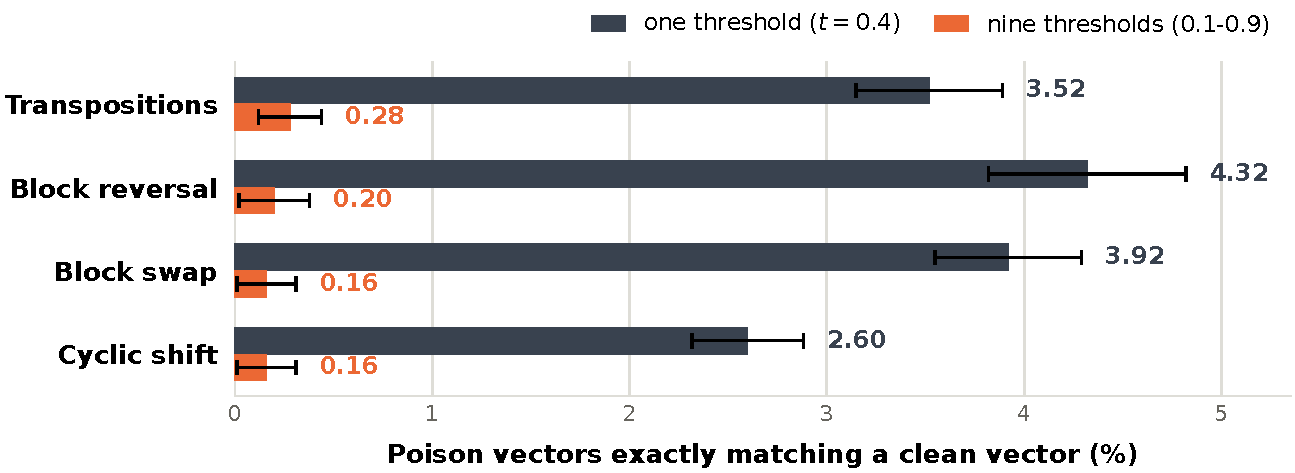
\includegraphics[width=0.88\textwidth]{figures/figure_v6_representation_repair.pdf}
  \caption{Exact feature-vector matches between poison and any clean row under
  the single-threshold control and the fixed nine-threshold stack. Bars show
  five-seed means; dots show individual seeds. The same attack realization is
  used in both arms.}
  \label{fig:repair}
\end{figure*}

The audit also separates equality from density behavior. Under the fixed
control, $\meanstd{42.28}{1.64}$\% of poison shares an exact final coordinate
with clean, while $\meanstd{56.24}{1.65}$\% is labeled OPTICS noise. Only
$\meanstd{1.80}{0.51}$\% is removed in a 100\%-poison cluster. Exact collisions
are therefore load-bearing under this fit, but the noise assignment affects a
larger portion of poisoned rows.

The strict-purity failure decomposition is exhaustive. Averaged over seeds,
39.48\% of poison is non-noise but shares a final vector with clean, 2.48\% is
non-noise and coordinate-distinct but lies in a mixed cluster, and the residual
unexplained category is exactly zero. No exact coordinate class is split across
two distinct non-noise OPTICS clusters. The only observed splits place some
identical members in one real cluster and others at label $-1$. Thus exact
coordinate sharing constrains this fit without being asserted as a universal,
algorithm-independent capture ceiling.

\subsection{The stack repairs identity but not detection}
The main comparison uses common eligible sources and guarantees a raw-changing
attack in every family--seed cell. Its control is therefore the matched
single-threshold arm for this new substrate, not the legacy provenance frame.
The nine-threshold representation sharply reduces the poisoned rows that
exactly match any clean feature vector (Fig.~\ref{fig:repair}). The reduction
is consistent across all four families and all five seeds: from 2.6--4.3\% in
the control to 0.2--0.3\% in the repair, a 13--20-fold decrease. In a paired
200-source diagnostic, the full stack also produces zero binary or 540-vector
identity for every family. Thus the intended algebraic repair succeeds.

That repair does not improve the primary endpoint. Table~\ref{tab:matched}
shows mean stack-minus-control poison-removal deltas at the five matched clean
costs. Through the $>0.80$ cutoffs, three families have exactly zero change;
cyclic shift is $-0.20$ percentage points, and block reversal is only $+0.64$
points, arising from one small cluster in three of five seeds. At the looser
$>0.50$ cutoff, every family is worse than control. No positive result is both
material and consistent across families.

\begin{table}[t]
\caption{Matched-clean-cost poison-removal delta (stack minus control)}
\label{tab:matched}
\centering
\scriptsize
\setlength{\tabcolsep}{3.1pt}
\begin{tabular}{lrrrrr}
\toprule
Family & 1.0 & $>.95$ & $>.90$ & $>.80$ & $>.50$ \\
\midrule
Transpositions & 0.000 & 0.000 & 0.000 & 0.000 & $-$.0188 \\
Block reversal & .0064 & .0064 & .0064 & .0044 & $-$.0060 \\
Block swap      & 0.000 & 0.000 & 0.000 & 0.000 & $-$.0152 \\
Cyclic shift    & $-$.0020 & $-$.0020 & $-$.0020 & $-$.0020 & $-$.0156 \\
\bottomrule
\end{tabular}
\end{table}

\begin{figure}[t]
  \centering
  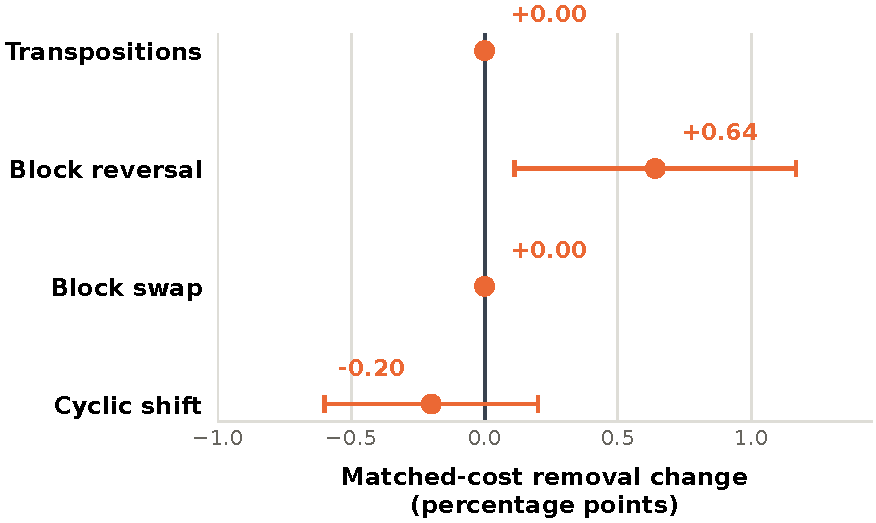
\includegraphics[width=\columnwidth]{figures/figure_v8_detector_outcome.pdf}
  \caption{Primary matched-clean-cost result at the strict control budget.
  Points are five-seed mean stack-minus-control poison-removal deltas; error
  bars are population SD. The small block-reversal effect corresponds to one
  poison-only cluster in three of five seeds.}
  \label{fig:detector}
\end{figure}

The downstream geometry explains the mismatch. In the control, poison noise is
85.2--87.5\% across families and clean noise is approximately 37.1--37.2\%.
With the stack, poison noise rises to 98.7--99.3\% and clean noise to
54.5--54.6\%; mean cluster count falls from 139.6--142.4 to 107.6--108.8.
The intervention separates exact coordinates but fragments the population
rather than forming removable poison-dominant clusters.

A paired diagnostic makes the statistical failure visible before clustering.
For 200 clean/source pairs per family, Table~\ref{tab:displacement} reports the
median attack displacement divided by the median displacement of ordinary
clean--clean pairings. Although the stack removes exact identity, its ratio is
smaller for every family. Moreover, zero of 200 attack displacements in either
representation exceed the corresponding clean--clean 95th percentile. The
repair therefore creates additional coordinates without making the attacks
unusual in the population metric used by OPTICS.

\begin{table}[t]
\caption{Attack-to-clean median displacement ratio}
\label{tab:displacement}
\centering
\scriptsize
\setlength{\tabcolsep}{4.2pt}
\begin{tabular}{lrrc}
\toprule
Family & Control & Stack & Above clean 95th \\
\midrule
Transpositions & .176 & .122 & 0/200 \\
Block reversal & .107 & .070 & 0/200 \\
Block swap      & .125 & .087 & 0/200 \\
Cyclic shift    & .139 & .107 & 0/200 \\
\bottomrule
\end{tabular}
\end{table}

\subsection{Deduplication changes degeneracy, not the conclusion}
Exact-payload deduplication reduces the 5,000-row clean frames to
$\meanstd{3974}{29}$ rows without backfill. As Table~\ref{tab:q4} shows, it
changes the raw stage's share of collision mass from 50.80\% to 5.49\% and
reduces final clean/poison coordinate obstruction by 5.34 percentage points.
Nevertheless, strict-purity poison capture falls by 1.44 points, while clean
and poison noise increase. Removing clean--clean raw repetition therefore does
not recover poisoned samples; it shifts more failure into OPTICS noise.

\begin{table}[t]
\caption{Separate exact-payload deduplication mechanism test}
\label{tab:q4}
\centering
\scriptsize
\setlength{\tabcolsep}{3.3pt}
\begin{tabular}{lrrr}
\toprule
Metric & Control & Deduplicated & $\Delta$ \\
\midrule
Raw collision-mass share & .5080 & .0549 & $-$.4531 \\
Final-vector obstruction & .4228 & .3694 & $-$.0534 \\
Poison noise             & .5624 & .6458 & +.0834 \\
Clean noise              & .3756 & .4541 & +.0785 \\
Strict-purity capture (\%) & 1.800 & .355 & $-$1.445 \\
\bottomrule
\end{tabular}
\end{table}

The label-free first-occurrence rule is not necessarily neutral: before
deduplication, $\meanstd{117.2}{5.2}$ repeated payload classes per seed contain
conflicting dataset labels. This supports treating Q4 only as a mechanism test,
not as a recommended preprocessing step.

The raw stage's collision-mass share is denominator-dependent. Deduplication
removes a large clean--clean repeated-class population, so that share falls
even though raw-no-op poison remains. Indeed, the poison rate whose earliest
merger is raw payload changes from 11.52\% to 13.06\%, rather than falling. The
intervention lowers final obstruction, but not in proportion to the 45.31-point
change in collision-mass attribution. This divergence is direct evidence that
population-level redundancy and poison-specific obstruction are different
quantities.

\section{Discussion}
The results establish a useful hierarchy of claims. At the \emph{algebraic}
level, the fixed stack closes the targeted single-threshold equality mechanism.
At the \emph{statistical} level, however, attack-induced displacement remains
small relative to ordinary clean--clean variation. At the \emph{detector}
level, OPTICS returns a more fragmented clustering and no matched-cost gain.
Success at the first level is therefore insufficient evidence for the second
or third.

The provenance audit also changes how the negative result should be assigned.
Approximately 97.5\% of repeated-member collision mass originates in either
the raw data or single-threshold mask, upstream of persistent homology. The
small diagram-stage component creates no new clean/poison mixed classes in the
audited frames, and the five filtration images and finite vector summaries add
no exact mergers. These observations do not show that TDA is injective or that
topology never loses attack information. They show that exact clean/poison
confusion in this fixed experiment is not primarily created by the
topological feature map.

Why does a representation with fewer exact matches perform no better? The
stack adds distinctions, but equal weighting does not guarantee that the new
coordinates emphasize attack-specific variation. On paired diagnostics,
attack displacement grows in absolute terms while its ratio to typical
clean--clean displacement falls. With the unchanged density radius, the
540-dimensional population becomes less clusterable, moving both groups to
label $-1$. Q4 produces the same qualitative lesson by a different route:
reducing duplicated population mass changes density support and increases
noise. Collision prevalence alone is therefore a poor proxy for usable poison
separation.

For security evaluation, this distinction prevents two tempting but invalid
inferences. First, a large raw-collision share does not mean that deduplication
will restore poison capture: most removed mass can be clean--clean density
support. Second, a large reduction in exact poison/clean matches does not mean
that a detector has become useful: the new positions may still lie in regions
that OPTICS treats as sparse. A defense claim should therefore report at least
one representation-level endpoint, one relative-separation endpoint, and one
operational endpoint with a clean-data cost. The stage-wise audit supplies the
first two diagnoses; (3) supplies the final comparison.

Several limitations bound the claims. First, Payload-Byte is a packet-level
derivative with padded payloads and inherited labels; conclusions need not
transfer to the original flow-level UNSW-NB15 tables or live traffic. Second,
the reconstruction fixes one recoverable interpretation of raster geometry and
feature assembly. Differences between the source paper's reported feature
count and the installed library's realized 60-feature output preclude an exact
reproduction claim. Third, five seeds quantify Monte Carlo stability but not
cross-dataset generalization. Fourth, the attacks are four structured,
guaranteed-nontrivial permutation families, not all possible transformations.
Finally, cluster purity is oracle information used only to compare removal
curves; a deployed system still needs a label-free rule for deciding which
clusters to reject.

These limits also define future work. A new preregistered study could test a
label-free anomaly score, a metric calibrated to clean traffic, or a second
dataset. Learned threshold weights, feature selection, alternative
filtrations, and OPTICS retuning may be reasonable designs, but using the
present outcomes to select them would convert a controlled test into post hoc
optimization. They are intentionally not evaluated here.

\section{Conclusion}
In this controlled reconstruction, a stage-wise audit locates nearly all exact
feature degeneracy before the topological summaries: in the legacy-transposition
provenance frame, 50.80\% of final
repeated-member collision mass is already raw-identical and 46.68\% first
merges at one binary cutoff. A fixed nine-threshold stack removes most exact
clean/poison feature matches, but it does not improve poison removal at matched
clean cost; instead, almost all poisoned rows become OPTICS noise. Removing
duplicate clean payloads likewise reduces degeneracy without restoring capture.
The contribution is thus not a stronger detector but a more defensible way to
evaluate one: localize information loss, separate representation repair from
population separation, and require downstream gains to survive a fixed-cost
comparison before claiming improved poisoning defense.

\clearpage
\balance
\begin{thebibliography}{10}

\bibitem{biggio2018}
B. Biggio and F. Roli, ``Wild patterns: Ten years after the rise of adversarial
machine learning,'' \emph{Pattern Recognition}, vol. 84, pp. 317--331, 2018,
doi: 10.1016/j.patcog.2018.07.023.

\bibitem{monkam2024}
C. Monkam, M. J. De Lucia, and N. D. Bastian, ``A topological data analysis
approach for detecting data poisoning attacks against machine learning based
network intrusion detection systems,'' \emph{Computers \& Security}, vol. 144,
Art. no. 103929, 2024, doi: 10.1016/j.cose.2024.103929.

\bibitem{carlsson2009}
G. Carlsson, ``Topology and data,'' \emph{Bulletin of the American Mathematical
Society}, vol. 46, no. 2, pp. 255--308, 2009,
doi: 10.1090/S0273-0979-09-01249-X.

\bibitem{cohensteiner2007}
D. Cohen-Steiner, H. Edelsbrunner, and J. Harer, ``Stability of persistence
diagrams,'' \emph{Discrete \& Computational Geometry}, vol. 37, no. 1,
pp. 103--120, 2007, doi: 10.1007/s00454-006-1276-5.

\bibitem{moustafa2015}
N. Moustafa and J. Slay, ``UNSW-NB15: A comprehensive data set for network
intrusion detection systems (UNSW-NB15 network data set),'' in \emph{Proc.
Military Communications and Information Systems Conf. (MilCIS)}, 2015,
pp. 1--6, doi: 10.1109/MilCIS.2015.7348942.

\bibitem{farrukh2022}
Y. A. Farrukh, I. Khan, S. Wali, D. Bierbrauer, J. A. Pavlik, and
N. D. Bastian, ``Payload-Byte: A tool for extracting and labeling packet
capture files of modern network intrusion detection datasets,'' in
\emph{Proc. IEEE/ACM Int. Conf. Big Data Computing, Applications and
Technologies (BDCAT)}, 2022, pp. 58--67,
doi: 10.1109/BDCAT56447.2022.00015.

\bibitem{tauzin2021}
G. Tauzin, U. Lupo, L. Tunstall, J. Burella P\'erez, M. Caorsi,
A. M. Medina-Mardones, A. Dassatti, and K. Hess, ``giotto-tda: A topological
data analysis toolkit for machine learning and data exploration,''
\emph{Journal of Machine Learning Research}, vol. 22, no. 39, pp. 1--6, 2021.

\bibitem{ankerst1999}
M. Ankerst, M. M. Breunig, H.-P. Kriegel, and J. Sander, ``OPTICS: Ordering
points to identify the clustering structure,'' in \emph{Proc. ACM SIGMOD Int.
Conf. Management of Data}, 1999, pp. 49--60,
doi: 10.1145/304182.304187.

\end{thebibliography}

\end{document}
